\chapter{Исследовательская часть}
В этом разделе будет продемонстрирована работа программы, а также
приведены результаты тестирования алгоритмов.

\section{Демонстрация работы программы}
На рисунке 4.1 приведена демонстрация работы программы.

\FloatBarrier
\begin{figure}[h]
	\begin{center}
		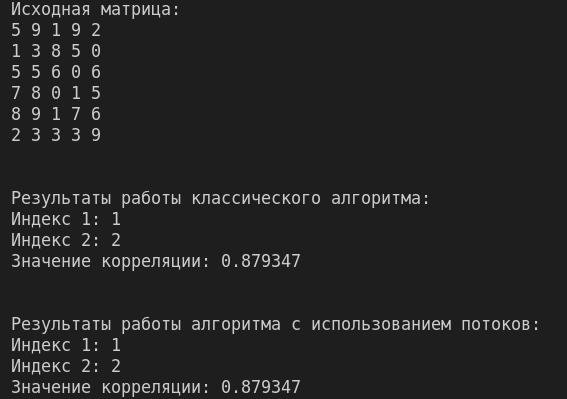
\includegraphics[]{inc/demonstrate.jpg}
	\end{center}
	\caption{Демонстрация работы программы}
\end{figure}
\FloatBarrier

\section{Технические характеристики}
Технические характеристики устройства, на котором выполнялось тестирование, следующие:
\begin{itemize}
	\item операционная система: Ubuntu 20.04.1 LTS;
	\item память: 8 GB;
	\item процессор: Intel Core i5-1135G7 @ 2.40GHz \cite{intel}.
	\item количество ядер процессора: 8
\end{itemize}

Во время тестирования ноутбук был нагружен только встроенными приложениями окружения, а также непосредственно системой тестирования.

\section{Тестирование программы}
Для определения быстродействия работы алгоритмов будет проведено исследование зависимости
на квадратных матрицах, так как её размер однозначно определяется по одной переменной. 

В таблице 4.1 представлены результаты тестирования времени работы алгоритма в зависимости от количества потоков и размера матрицы.
Время - в микросекундах.

\FloatBarrier
\begin{table}[h]
	\caption{Результаты тестов (с учётом того, что один поток - главный)}
	\centering
	\begin{tabular}{ | l | l | l | l | l | l | l |}
		\hline
		Размер & Классический & 2 потока & 4 потока & 8 потоков & 16 потоков & 32 \\ \hline
		2 & 1 & 44 & 79 & 219 & 226 & 223 \\
		5 & 4 & 52 & 103 & 294 & 287 & 272\\
		10 & 11 & 81 & 157 &  324 & 835 & 602 \\
		25 & 104 & 240 & 225 & 444 & 892 & 901 \\
		50 & 673 & 1014 & 690 & 741 & 1162 & 1225 \\
		75 & 2181 & 2811 & 2025 & 1676 & 2195 & 2215 \\
		100 & 5242 & 6575 & 4328 & 3491 & 4291 & 4181\\
		200 & 45820 & 51614 & 32406 & 22376 & 21584 & 21769 \\
		500 & 777738 & 798849 & 491472 & 378796 & 316299 & 363662 \\
		750 &  3765498 & 4036732 & 2285193 & 1535681 & 1419432 & 1492165\\
		1000 & 7883329 & 8551277 & 4943219 & 3264990 & 3070650 & 3105601 \\
		\hline
	\end{tabular}
\end{table}
\FloatBarrier
На рисунке 4.1 показан график зависимости времени работы алгоритмов от размера матрицы и количества потоков.

\FloatBarrier
\begin{figure}[h]
	\begin{center}
		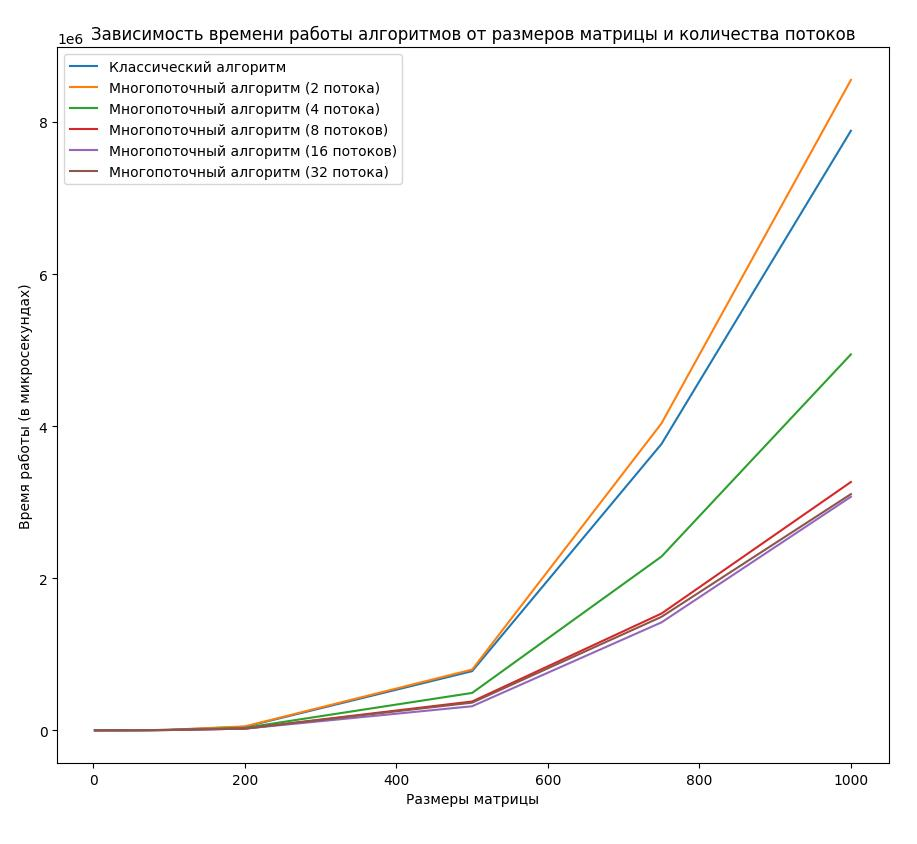
\includegraphics[width=\linewidth]{inc/result.jpg}
	\end{center}
	\caption{График зависимости времени работы алгоритмов от размера матрицы и количества потоков}
\end{figure}
\FloatBarrier

На 16 потоках программа показала наилучшие результаты.

\section{Вывод}
Распараллеливание программы действительно привело к ускорению работы программы.

На матрице размером $N=1000$ 16-поточный алгоритм показал наилучшие результаты, опередив на 20\% 8-поточный алгоритм, в полтора раза
алгоритм c $M=4$ потоками, и в 2.5 раза - классический и двухпоточный алгоритмы. Такие же пропорции наблюдаются
при $N=500$, $N=200$. При $N=100$ 8-поточный алгоритм занял первое место.

На матрице размером $N <= 50$ классический алгоритм показал наилучшие результаты. Это связано с тем,
что поддержка потоков также требует дополнительных системных ресурсов, и для маленьких матриц это оказалось
неэффективным. Но при матрицах $N > 50$ многопоточные алгоритмы уже оправдывают ожидания.

Алгоритм с двумя потоками оказался самым медленным при $N >=50$. Это объясняется тем, что в реализации
один из потоков - главный, и он лишь ждёт выполнения работы другим потоком. То есть это был такой же 
классический алгоритм, но при этом он поддерживал многопоточность, то есть системные затраты были выше.

Увеличения числа потоков в два раза не привело к уменьшению работы программы в два раза. Для
$M_1 = 2$ и $M_2 = 4$ в среднем четырёхпоточный показал время в 1.8 раз меньше. Для 
$M_1 = 4$ и $M_2 = 8$ разница составила 50 \%. Такого ускорения не было, потому что потоки чаще 
обращаются к сравнению глобальной переменной, и мьютекс блокирует доступ к переменным. Более того,
у самих потоков становится меньше системных ресурсов, поэтому выполнение потока по отдельности
происходит медленнее.

В случае $M_1 = 8$ и $M_2 = 16$ вообще не наблюдается выигрыша до $N=200$, а затем 16-поточный алгоритм стал 
работать быстрее на 20\%. При этом в случае превышения количеством потоков количества логических ядер,
выигрыша по времени не наблюдается, что заметно по поведению графика для $M_1 = 16$ и $M_2 = 32$.
При таком превышении растёт нагрузка на процессор, но выигрыша не наблюдается, поэтому можно сделать вывод,
что такое число потоков не является эффективным.

Затраты на память у обоих алгоритмов имеют один и тот же порядок $O(N)$.